\documentclass[%
	11pt,
	a4paper,
	utf8,
	%twocolumn
		]{article}	

\usepackage{style_packages/podvoyskiy_article_extended}


\begin{document}
\title{Сборник заметок\\по использованию Kubernetes в контексте машинного обучения}

\author{}

\date{}
\maketitle

\thispagestyle{fancy}

\tableofcontents


\section{Основные термины}

\noindent\emph{под} (pod) -- группа \emph{контейнеров} (один или несколько); минимальная сущность, управляемая Kubernetes; у всех контейнеров внутри одного пода общие network, IPC, UTS, PID*, namespace; pod нельзя делить между узлами кластера \pic{fig:pod}; на \pic{fig:podpatterns} приведены основные паттерны использования подов

\begin{figure}[h]
	\centering
	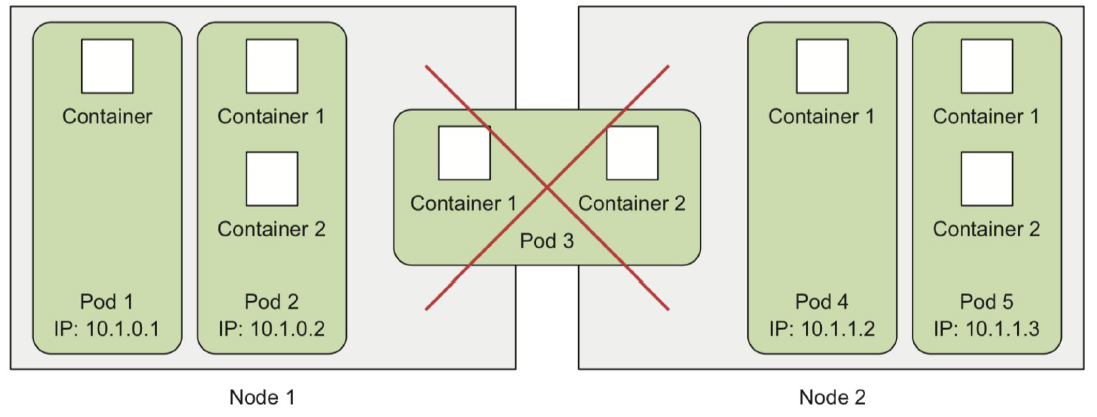
\includegraphics[scale=0.55]{figures/pod.png}
	\caption{ Иллюстрация концепции подов }\label{fig:pod}
\end{figure}

\begin{figure}[h]
	\centering
	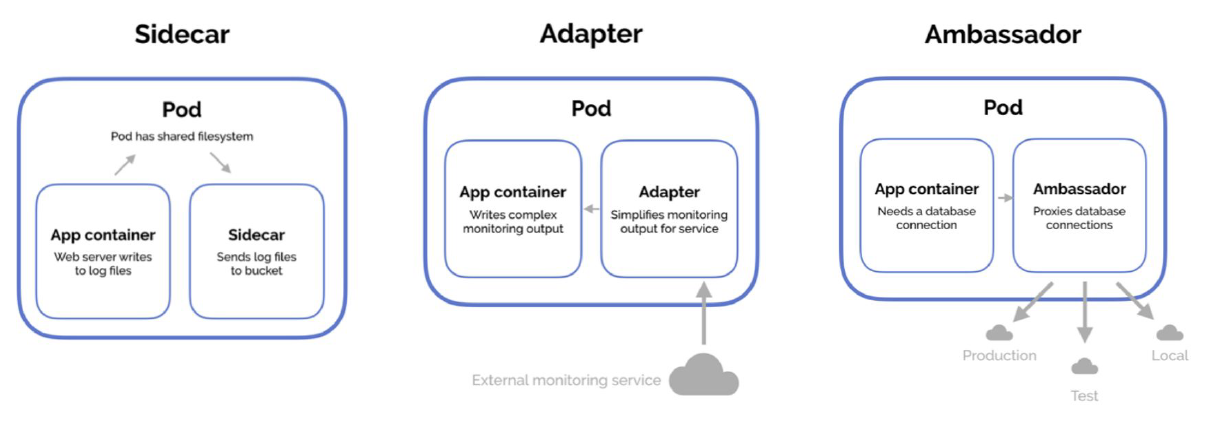
\includegraphics[scale=0.55]{figures/podpatterns.png}
	\caption{ Паттерны использования подов }\label{fig:podpatterns}
\end{figure}


\section{Общие замечания}

Для небольших проектов из нескольких контейнеров удобнее использовать оркестратор Nomad \url{https://www.nomadproject.io/}.

Кластер Kubernetes состоит из набора \emph{машин}, так называемых \emph{узлов}, которые запускают контейнеризированные приложения. Кластер должен иметь как минимум один рабочий узел.

На рабочих узлах размещены поды (pod's), являющиеся компонентами приложения. Внутренние сервисы Kubernetes управляют рабочими узлами и подами в кластере. Сервисы обычно запускаются на нескольких компьютерах, а кластер, как правило, развертывается на нескольких узлах, гарантируя отказоустойчивость и высокую надежность.

Например, в Mail Cloud Solutions топология кластеров включает в себя понятие мастер-узлов, на которых располагаются управляющие сервисы, и групп рабочих узлов, на которых запускаются приложения пользователя. Каждый кластер Kubernetes может содержать несколько групп рабочих узлов, каждая из которых создана на базе определенного шаблона виртуальной машины.


\section{Начало работы в Kubernetes с помощью Minikube}

Для работы с Kubernetes система должна поддреживать виртуализацию. На MacOS X это можно проверить так
\begin{lstlisting}[
style = bash,
numbers = none
]
sysctl -a | grep machdep.cpu.features | grep VMX
\end{lstlisting}

Если возвращается непустой результат, то можно продолжать. Теперь требуется установить гипервизор, например, VirtualBox \url{https://www.virtualbox.org/wiki/Downloads}.

Далее требуется установить \texttt{minikube}. На Mac OS X это можно сделать с помощью менеджера \texttt{brew}
\begin{lstlisting}[
style = bash,
numbers = none	
]
brew install minikube
\end{lstlisting}

\texttt{minikube} -- утилита командной строки для настройки и запуска \emph{одноузлового кластера Kubernetes} в виртуальной машине на \emph{локальном} компьютере. Этот вариант идеально подходит для первого знакомства с кластером под управлением Kubernetes и выполнения простых операций.

Проверка установки
\begin{lstlisting}[
style = bash,
numbers = none	
]
minikube start --vm-driver=virtualbox
minikube status
\end{lstlisting}

Если кластер запущен, то в выводе команды \texttt{minikube status} должно быть что-то вроде
\begin{lstlisting}[
style = bash,
numbers = none	
]
host: Running
kubelet: Running
apiserver: Running
kubeconfig: Configured
\end{lstlisting}

Вместе с \texttt{minikube} устанавливается и утилита \texttt{kubectl} для работы с полноценным кластером под управлением Kubernetes.

Можно посмотреть список запущенных в кластере подов (групп контейнеров) и нод
\begin{lstlisting}[
style = bash,
numbers = none	
]
kubectl get pods --all-namespaces
kubectl get nodes
\end{lstlisting}

Теперь можно запустить встроенный под \texttt{hello-minikube}. Для этого пода будет создан предварительно настроенный deployment
\begin{lstlisting}[
style = bash,
numbers = none	
]
kubectl run hello-minikube --image=gcr.io/google_containers/echoserver:1.4 --port=8080 # pod/hello-minikube created
\end{lstlisting}

Можно снова посмотреть на актуальные списки подов
\begin{lstlisting}[
style = bash,
numbers = none	
]
kubectl get pods
\end{lstlisting}

Удалить под и ноду
\begin{lstlisting}[
style = bash,
numbers = none	
]
kubectl delete pod hello-minikube
kubectl delete node minikube
\end{lstlisting}

\section{Процедура развертывания веб-приложения в Kubernetes с нуля}

\url{https://habr.com/ru/articles/752586/}

\url{https://habr.com/ru/articles/444446/}

Основные типы ресурсов:
\begin{itemize}
	\item \verb*|Pod|: одноразовая, очень нестабильная сущность,
	
	\item \verb*|ReplicaSet|: следит за тем, чтобы было создано указанное количество подов,
	
	\item \verb*|Deployment|: упрощает процедуру обновления подов; деплоймент создает репликасет, который порождает заданное количество подов,
	
	\item \verb*|StatefulSet|: создает упорядоченный набор подов с фиксированными именами (следовательно, с адресами, по которым можно обращаться к ним внутри кластера).
\end{itemize}

В случае разворачивания простых и слабо нагруженных проектов в целом можно просто делать \verb|docker compose up -d| на продакш-сервере и это будет работать. Но как только продакш-серверов становится больше одного, это, конечно, резко перестает быть удобно.

Поднятие кластера Kubernetes с нуля -- нетривиальная задача и, как правило, удел команды DevOps. Но существует множество решений, позволяющих поднять кластер на несколько нод за небольшую плату (например, DigitalOcean). 

Потребуется установить \verb*|kubectl| -- это утилита командной строки для работы с кластером Kubernetes.

Все, что происходит в кластере Kubernetes, описывается через создание и изменение ресурсов разных типов. Собственно, большая часть операций \verb*|kubectl| сводится к CRUD-операциям над ресурсами.

Для удобства ресурсы рассортированы по пространствам имен (namespace). Пространство имен это тоже ресурс. Запросить список ресурсов можно так
\begin{lstlisting}[
style = bash,
numbers = none
]
$ kubectl get namespaces
# output
NAME              STATUS   AGE
default           Active   1d
kube-node-lease   Active   1d
kube-public       Active   1d
kube-system       Active   1d
\end{lstlisting}

С точки зрения пользователя кластера Kubernetes ресурсы -- это просто файлы YAML/JSON. Командой \verb|kubectl get| можно получить YAML для конкретного ресурса -- например, для default
\begin{lstlisting}[
style = bash,
numbers = none
]
$ kubectl get namespace -o yaml default
# output
apiVersion: v1
kind: Namespace  # тип ресурса
metadata:
	creationTimestamp: "2022-07-25T18:00:57Z"
	labels:
		kubernetes.io/metadata.name: default
	name: default
	resourceVersion: "200"
	uid: 492e34b7-82e0-472b-9fb9-3ed7005a83eb
spec:
	finalizers:
	- kubernetes
status:
	phase: Active
\end{lstlisting}

Поле \verb*|kind| содержит тип ресурса. \verb|-o yaml| это формат вывода. Еще бывает полезен \verb|-o json|
\begin{lstlisting}[
style = bash,
numbers = none
]
$ kubectl get namespace -o json default | jq .status.phase  # "Active"
# можно использовать короткие псевдонимы
$ kubectl get ns -o json default ...
\end{lstlisting}

\emph{Под} -- минимальная единица выполнения в Kubernetes. Под -- это несколько (или даже один) Docker-контейнеров, гарантировано запускаемых на одном узле (ноде) виртуальной машины, так как поды нельзя делить между узлами кластера. В простейшем случае это один контейнер, в котором крутится сервис; другой типичный сценарий -- один контейнер с сервисом и второй, например, с обработчиком логов вроде Filebeat.

Для примера создадим под со встроенным в Python HTTP-сервером
\begin{lstlisting}[
style = bash,
numbers = none
]
$ kubectl apply -f - <<EOF
apiVersion: v1
kind: Pod
metadata:
  name: test-pod
spec:
  containers:
    - name: python-container
    image: python:bullseye
    command: ["python3", "-m", "http.server", "8080"]
EOF
\end{lstlisting}

Можно сохранить YAML в файл и затем вызвать
\begin{lstlisting}[
style = bash,
numbers = none
]
$ kubectl apply -f path/to/filename.yaml  # pod/test-pod created
\end{lstlisting}

Вывести список подов можно так
\begin{lstlisting}[
style = bash,
numbers = none
]
kubectl get pods
\end{lstlisting}

При создании под Kubernetes выбрал на какой ноде разместить под. Затем стянул (pull) на эту ноду указанный Docker-образ. Затем создал контейнер и запустил его.

По аналогии с \verb|docker exec| мы можем запускать команды в контейнерах через \verb*|kubectl exec|, в том числе в интерактивном режиме
\begin{lstlisting}[
style = bash,
numbers = none
]
$ kubectl exec test-pod -- whoami  # root
$ kubectl exec -it test-pod -- /bin/bash
\end{lstlisting}

Проверим, что HTTP-сервер в нашем поде действительно работает, получив к нему локальный доступ
\begin{lstlisting}[
style = bash,
numbers = none
]
$ kubectl port-forward pod/test-pod 7080:8080
\end{lstlisting}

Теперь можно открыть \verb|http://localhost:7080/| и увидеть стандартный ответ \verb*|http.server|.

Можно посмотреть логи контейнера
\begin{lstlisting}[
style = bash,
numbers = none
]
kubectl logs test-pod
\end{lstlisting}

Собираем Docker-образы
\begin{lstlisting}[
style = bash,
numbers = none
]
$ docker build --target backend -t habr-app-demo/backend:latest backend
$ docker build --target worker -t habr-app-demo/worker:latest backend
$ docker build -t habr-app-demo/frontend:latest frontend
\end{lstlisting}

Если бы у нас был настоящий продакшн-кластер Kubernetes, где-то радом с ним было бы корпоративное хранилище Docker-образов, в которое было бы достаточно их запушить. Например, если бы мы завели \emph{хранилище} под названием \verb*|habr-app-demo-registry| в DigitalOcean, это выглядело бы так
\begin{lstlisting}[
style = bash,
numbers = none
]
# создаем псевдоним для образа habr-app-demo/backend:latest
$ docker tag \
    habr-app-demo/backend:latest \
    registry.digitalocean.com/habr-app-demo-registry/backend
$ docker push registry.digitalocean.com/habr-app-demo-registry/backend
\end{lstlisting}

Теперь можно имя \verb*|registry.digitalocean.com/habr-app-demo-registry/backend:latest| использовать как имя образа в поде.

Если мы хотим продолжить работать с \verb*|minikube|, не подключая платные облачные решения, нужно использовать \verb|minikube docker-env|. \verb*|minikube| поднимает свой собственный Docker deamon и образы нужно собирать в нем, чтобы Kubernetes мог найти их локально
\begin{lstlisting}[
style = bash,
numbers = none
]
eval $(minikube docer-env)
docker build --target backend -t habr-app-demo/backend:latest backend
docker build --target worker -t habr-app-demo/worker:latest backend
docker build -t habr-app-demo/frontend:latest frontend
\end{lstlisting}

Поды задуманы как одноразовые, неустойчивые сущности: кластер Kubernetes может удалить любой под в любой момент. Для создания стабильного набора подов Kubernetes предоставляет другой низкоуровневый тип ресурса -- \verb*|ReplicaSet|. Репликасет позволяет указать количество желаемых подов и шаблон, по которому можно клепать эти поды.
\begin{lstlisting}[
style = bash,
numbers = none
]
apiVersion: apps/v1
kind: ReplicaSet
metadata:
	name: backend-replicaset
spec:
	replicas: 2  # сколько подов нужно держать поднятыми

	# template -- шаблон для создания подов. Содержимое по синтаксису
	# аналогично описанию пода (см. пример выше), с небольшими различиями:
	# apiVersion и kind не нужно указывать -- и так понятно, что
	#   это под в той же версии API, что и репликасет;
	# также не нужно указывать name -- он будет генерироваться
	#   движком Kubernetes исходя из названия репликасета.
	template:
		metadata:
			# labels -- это произвольные key-value пары, хранящие 
			# метаинформацию о поде. Выбор ключа app и значения 
			# backend-app произволен. Но этот лейбл потребуется нам ниже!
			labels:
				app: backend-app

		spec:
			containers:
				- name: backend-container

					# Способ указать minikube использовать ранее собранные
					# нами локально образы. Без настройки imagePullPolicy
					# Kubernetes будет пытаться тянуть образ из интернета 
					# (и, конечно, не сможет его найти и сфейлится).
					image: docker.io/habr-app-demo/backend:latest
					imagePullPolicy: Never

					ports:
					- containerPort: 40001

	# selector -- это способ для репликасета понять, какие поды
	# из числа уже существующих в кластере относятся к нему. Поскольку
	# мы прописали в шаблоне выше лейбл app: backend-app, мы точно
	# знаем, что все поды с таким лейблом порождены этим репликасетом.
	# Репликасет будет пользоваться этим селектором, чтобы понять,
	# сколько он уже насоздавал подов и сколько ещё нужно, чтобы 
	# добиться количества реплик, указанного выше в поле replicas.
	selector:
		matchLabels:
			app: backend-app
\end{lstlisting}

Занимается репликасет исключительно тем, что создает и поддерживает нужное количество активных подов -- рестартует поды при наличие ошибок, создает новые в случае удаления (например, в сценарии с падением ноды или если вы решите удалить один из подов руками и т.д.).

Мы могли бы создать репликасет по YAML выше и увидеть как создает два пода. Но у репликасет есть минус -- неудобно обновлять поды. Нам бы хотелось, чтобы если версия бекэнда обновится, она выкатывалась постепенно, под за подом. С репликасетами же нам придется вручную создавать новый репликасет с актуальной версией и либо разом удалять старый (что под нагрузкой опасно), либо менять \verb*|replicas| в обоих репликасетах, сдувая старый и надувая новый. К счастью, есть более высокоуровневый компонент, умеющий заниматься ровно этим.

Для удобного развертывания сервисов в Kubernetes есть ресурс \verb*|Deployment|, для создания которого нужно указать все те же параметры, что и для репликасетов, плюс (опционально) настройки той самой плавной выкатки -- например, какое максимальное количество подов может быть в переходном состоянии в каждый момент времени.

Поведение деплоймента в общих чертах выглядит так. При создании деплоймент создает репликасет, который порождает нужное количество подов и берется следить, чтобы их количество не менялось. Это распространенный шаблон Kubernetes -- высокоуровневые абстракции создают низкоуровневые, чтобы реализовать поверх них более сложное поведение. Далее, при необходимости перевыкатки деплоймент возьмет на себя создание второго репликасета и постепенное масштабирование их обоих до тех пор, пока в старом не останется подов.
\begin{lstlisting}[
style = bash,
numbers = none
]
# k8s/backend-deployment.yaml
apiVersion: apps/v1
kind: Deployment
metadata:
	name: backend-deployment
spec:
	replicas: 2
	template:
		metadata:
			labels:
				app: backend-app
		spec:
			containers:
				- name: backend-container
				image: docker.io/habr-app-demo/backend:latest
				imagePullPolicy: Never
				ports:
					- containerPort: 40001
	selector:
		matchLabels:
			app: backend-app
\end{lstlisting}

Создадим деплоймент
\begin{lstlisting}[
style = bash,
numbers = none
]
$ kubectl apply -f k8s/backend-deployment.yaml  # deployment.apps/backend-deployment created
\end{lstlisting}

Список ресурсов
\begin{lstlisting}[
style = bash,
numbers = none
]
$ kubectl get all
# output
NAME                                    READY STATUS           RESTARTS    AGE
pod/backend-deployment-77cc555f4b-2wv24 0/1   CrashLoopBackOff 2 (19s ago) 45s
pod/backend-deployment-77cc555f4b-kd4k9 0/1   CrashLoopBackOff 2 (18s ago) 44s
pod/test-pod                            1/1   Running          0           1h

NAME                               READY UP-TO-DATE AVAILABLE AGE
deployment.apps/backend-deployment 0/2   2          0         50s

NAME                                          DESIRED CURRENT READY AGE
replicaset.apps/backend-deployment-77cc555f4b 2       2       0     47s
\end{lstlisting}

Случилось ровно то, что и ожидалось -- создался деплоймент, он породил репликасет с названием, сгенерированным по названию деплоймента, а уже в рамках этого репликасета создались два пода с названиями сгенерированными по названию репликасета.

<<\verb*|CrashLoopBackOff|>> значит, что Kubernetes создал поды, но контейнеры в них падают с ошибкой, и делают это раз за разом. Если бы контейнер упал один раз, у него был бы статус \verb*|Error|, быстро сменяющийся рестартом.

Смотрим логи произвольного пода из деплоймента 
\begin{lstlisting}[
style = bash,
numbers = none
]
$ kubectl logs deployment/backend-deployment
# output
Found 2 pods, using pod/backend-deployment-77cc555f4b-2wv24
...
pymongo.errors.ServerSelectionTimeoutError: mongo:27017: [Errno -2] Name does not resolve, Timeout: 1.0s, Topology Description: <TopologyDescription id: 64a319b1d732cacfbcdd43f1, topology_type: Unknown, servers: [<ServerDescription ('mongo', 27017) server_type: Unknown, rtt: None, error=AutoReconnect('mongo:27017: [Errno -2] Name does not resolve')>]>
...
\end{lstlisting}

Очевидно, не поднята база данных. Грамотно развернуть базу данных в промышленной среде -- весьма нетривиальная задача, и нет общего мнения, что делать это в кластере Kubernetes -- хорошая идея. Как правило, облачные провайдеры предоставляют свои SaaS-решения для разворачивания самых популярных БД и они будут куда надежнее, чем результаты самодеятельности.

Поды не очень стабильные объекты, создаваемые и удаляемые по прихоти Kubernetes-кластера. Под может быть размещен на любой подходящей ноде кластера (но этим можно управлять). При этом у пода генерируется непредсказуемый ID, и обратиться к нему извне становится сложно, как и, например, понять внутри самого пода, кто он: главная реплика базы данных, вторичная и пр.

Поэтому для stateful-сервисов Kubernetes предоставляет отдельную абстракцию -- \verb*|StatefulSet|, позволяющую создавать относительно стабильный и \emph{упорядоченный набор подов} с \emph{фиксированными} именами (и соответственно адресами, по которым можно обращаться к ним внутри кластера) и доступом к персистентым томам.

Создадим простейший StatefulSet, поднимающий одну реплику MongoDB
\begin{lstlisting}[
style = bash,
numbers = none
]
# k8s/mongodb-statefulset.yaml
apiVersion: apps/v1
kind: StatefulSet
metadata:
	name: mongodb-statefulset
spec:
	serviceName: mongodb-service
	replicas: 1  # сколько подов требуется в стейтфулсете
	template:
		metadata:
			labels:
				# label нужен из тех же соображений, что и в деплойменте.
				app: mongodb-app
		spec:
			containers:
				- name: mongodb-container
				image: mongo:6.0.6
	
				# Выставляем наружу дефолтный порт монги.
				ports:
				- containerPort: 27017
				name: mongodb-cli

	# selector нужен из тех же соображений, что и в деплойменте.
	selector:
		matchLabels:
			app: mongodb-app
\end{lstlisting}

Чтобы файлы базы данных сохранялись при создании подов, нужно примонтировать персистентное хранилище. Персистентные тома в Kubernetes создаются посредством ресурса \verb*|PersistentVolumne|, в котором можно указать размер, тип хранилища (в разных облаках доступны разные типы), политику монтирования (можно ли монтировать том строго на одной ноде или на нескольких) и пр. Тома привязываются к подам посредством промежуточного ресурса \verb*|PersistentVolumeClaim| (PVC), в котором можно указать требования к тому.

Поскольку в стейфулсете в общем случае больше одного пода и чаще всего разным подам нужны отдельные тома, сейтфулсет предоставляет возможность задать шаблон PVC, по которому \emph{на каждый созданный под будет создан свой том}
\begin{lstlisting}[
style = bash,
numbers = none
]
# k8s/mongodb-statefulset.yaml
	...
		containers:
			- name: mongodb-container
				...
				# Монтируем том с данными.
				volumeMounts:
					- mountPath: "/data/db"
					name: mongodb-pvc
	...
volumeClaimTemplates:
	- metadata:
			name: mongodb-pvc
	spec:
		accessModes:
			- ReadWriteOnce # можно читать/писать только на одной ноде
		resources:
			requests:
				storage: 100Mi
\end{lstlisting}

Создаем statefulset 
\begin{lstlisting}[
style = bash,
numbers = none
]
$ kubectl apply -f k8s/mogodb-statefulset.yaml  # statefulset.apps/mongodb-statefulset created
$ kubectl get pods
# output
NAME                                  READY  STATUS            RESTARTS        AGE
backend-deployment-77cc555f4b-2wv24   0/1    CrashLoopBackOff  42 (2m9s ago)   4h20m
backend-deployment-77cc555f4b-kd4k9   0/1    CrashLoopBackOff  42 (2m11s ago)  4h20m
# у пода mongodb неслучайный суффикс 
mongodb-statefulset-0                 1/1    Running           0               5s
test-pod                              1/1    Running           0               4h20m
\end{lstlisting}

Обратите внимание, что вместо случайного суффикса название пода оканчивается на порядковый номер пода в стейтфулсете, то есть при пересоздании номер пода гарантированно останется таким же.

В списке персистентных томов также видим автоматически созданный том
\begin{lstlisting}[
style = bash,
numbers = none
]
$ kubectl get persistentvolumes
# output
NAME                                     CAPACITY ACCESS MODES RECLAIM POLICY STATUS CLAIM                                     STORAGECLASS REASON AGE
pvc-88da024c-31ef-49f8-9b0b-3403bc3795d2 100Mi    RWO          Delete         Bound  default/mongodb-pvc-mongodb-statefulset-0 standard            13d
\end{lstlisting}

Теперь хорошы бы как-то проверить, что MongoDB работает; что можно к ней подключиться изнутри кластера, поделать запросы и пр. Но какой адрес у пода внутри кластера?

Для сетевого доступа к подам нам потребуется еще одна абстракция -- \verb*|Service|. Описание сервиса состоит из селектора подов, к которым нужно обеспечить доступ, и тип доступа. Поскольку нам нужен внутренний доступ к одному конкретному поду в StatefulSet, нас устроит самый простой тип сервиса, так называемый headless service -- без балансировки нагрузки и выделения статического IP для доступа извне
\begin{lstlisting}[
style = bash,
numbers = none
]
# k8s/mongodb-service.yaml
apiVersion: v1
kind: Service
metadata:
	name: mongodb-service
spec:
	# ClusterIP -- самый простой тип сервиса, который 
	# позволяет подам связываться друг с другом в рамках
	# кластера, но абсолютно никак не виден снаружи:
	type: ClusterIP
	clusterIP: None
	selector:
		app: mongodb-app
\end{lstlisting}

\begin{lstlisting}[
style = bash,
numbers = none
]
$ kubectl apply -f k8s/mongodb-service.yaml
\end{lstlisting}

Теперь для доступа к поду с БД внутри кластера должен заработать URL
\begin{lstlisting}[
style = bash,
numbers = none
]
$ <pod name>.<service name>.<namespace>.svc.cluster.local
\end{lstlisting}

То есть в нашем случае 
\begin{lstlisting}[
style = bash,
numbers = none
]
statefulset-0.mongodb-service.default.svc.cluster.local
\end{lstlisting}

Проверим, зайдя в тестовый под и попытавшись подключиться через pymongo
\begin{lstlisting}[
numbers = none
]
$ kubectl exec -it test-pod -- /bin/bash
/# python -m pip install pymongo
...
>>> import pymongo
>>> uri = "mongodb://mongodb-statefulset-0.mongodb-service.default.svc.cluster.local"
>>> c = pymongo.MongoClient(uri)
>>> c.some_database.some_collection.insert_one({"foo": "bar})
>>> list(c.some_database.some_collection.find({}))  # Работает!
\end{lstlisting}

Проверив поды бекэнда, мы заметим, что они все еще в \verb*|CharshLoopBackOff|, поскольку ожидают, что хостнейм монги -- \verb*|mongo|, как это было раньше, в решении с Docker Compose. Менять файл \verb*|k8s/backend-deployment.yaml| и пересоздавать деплоймент целиком не очень удобно; давайте внесем точечное изменение командой \verb|kubectl patch|
\begin{lstlisting}[
style = bash,
numbers = none
]
# k8s/backend-deployment-patch.yaml
spec:
	template:
		spec:
			containers:
				- name: backend-container
				env:
					- name: APP_ENV
					value: k8s
\end{lstlisting}

\begin{lstlisting}[
style = bash,
numbers = none
]
$ kubectl patch deployment backend-deployment \
    --patch-file k8s/backend-deployment-patch.yaml
\end{lstlisting}

Удобной альтернативой \verb|kubectl patch| может быть \verb|kubectl edit|, а также в этом конкретном случае настройки переменной окружения
\begin{lstlisting}[
style = bash,
numbers = none
]
$ kubectl set env deployment/backend-deployment APP_ENV=k8s
\end{lstlisting}

Смотрим ресурсы
\begin{lstlisting}[
style = bash,
numbers = none
]
$ kubectl get pods
# output
NAME                                 READY  STATUS   RESTARTS  AGE
backend-deployment-7547fb8b7c-4k2x7  1/1    Running  0         11s
backend-deployment-7547fb8b7c-hhvhd  1/1    Running  0         8s
...
\end{lstlisting}

Для хранения паролей и прочей приватной информации Kubernetes предоставляет еще один тип ресурсов -- \verb*|Secret|. Генерируем пароль и создаем секрет
\begin{lstlisting}[
style = bash,
numbers = none
]
echo -n "$(openssl rand -hex 14)" > password.txt
$ kubectl create secret generic mongodb-secret --from-file password.txt
\end{lstlisting}

В данном случае мы создали секрет, который можно будет подключать к контейнерам как раздел, в который будут подтягиваться исходные файлы.

Поправим конфигурацию MongoDB, чтобы у пользователя root был сгенерированный нами пароль. Конкретно в случае MongoDB это можно сделать, поправив переменную окружения \verb*|MONGO_INITDB_ROOT_PASSWORD_FILE|. Также нам нужно будет примонтировать раздел с файлом \verb*|password.txt|
\begin{lstlisting}[
style = bash,
numbers = none
]
# k8s/mongodb-statefulset-v2.yaml
...
	- env:
		...
			- name: MONGO_INITDB_ROOT_PASSWORD_FILE
			value: "/run/secrets/mongodb/password.txt"
		...
	
		# В разделе volumeMounts мы описываем, какие тома
		# по каким путям нужно примонтировать. Тома могут
		# иметь разное происхождение (например, сейчас у нас 
		# один персистентный том и один томик с секретами).
		# Описание того, какого типа какой том, вынесено в 
		# отдельное поле -- volumes (ниже).
		volumeMounts:
			- mountPath: "/data/db"
				name: mongodb-pvc
			- mountPath: "/run/secrets/mongodb"
				name: mongodb-secret-volume
				readOnly: true
		...
		# В разделе volumes мы описываем тома, которые нужно
		# примонтировать в соответствии с инструкциями в поле
		# volumeMounts.
		volumes:
			- name: mongodb-secret-volume
				# Указываем, что данные для этого тома надо взять
				# из ресурса Secret с названием mongodb-secret.
				secret:
					secretName: mongodb-secret
					optional: false
			# А персистентный том не надо описывать -- Kubernetes
			# сделает это за нас для всех подов в стейтфулсете.
...
\end{lstlisting}

Поскольку пароль берется во внимание только при инициализации базы данных с нуля, нам проще всего полностью удалить стейтфулсет и все данные и создать заново с новыми настройками (НЕ ПОВТОРЯТЬ на ПРОДЕ!!!)
\begin{lstlisting}[
style = bash,
numbers = none
]
# Удаляем стейтфулсет (а с ним и под)
$ kubectl delete statefulset mongodb-statefulset
# statefulset.apps "mongodb-statefulset" deleted

# Удаляем PersistentVolumeClaim, чтобы Kubernetes разрешил удалить сам том
$ kubectl delete pvc mongodb-pvc-mongodb-statefulset-0 
# persistentvolumeclaim "mongodb-pvc-mongodb-statefulset-0" deleted

$ kubectl get persistentvolumes
# No resources found

# Пересоздаём всё созданием нового стейтфулсета
$ kubectl apply -f k8s/mongodb-statefulset-v2.yaml
# statefulset.apps/mongodb-statefulset created
\end{lstlisting}

Если сейчас перезапустить поды бекэнда (например, командной \verb|kubectl rollout restart deployment|), увидим, что они снова попали в \verb*|CrashLoopBackOff| -- так как теперь нужен пароль. Нужно обновить \verb*|APP_ENV| и примонтировать секрет
\begin{lstlisting}[
style = bash,
numbers = none
]
# k8s/backend-deployment-patch-2.yaml
spec:
	template:
		spec:
			containers:
				- name: backend-container
					env:
						- name: APP_ENV
						value: k8s_secrets
					volumeMounts:
						- mountPath: "/run/secrets/mongodb"
							name: mongodb-secret-volume
							readOnly: true
			volumes:
				- name: mongodb-secret-volume
					secret:
						secretName: mongodb-secret
						optional: false
\end{lstlisting}

Применяем патч и видим, что вновь созданные поды работают без проблем
\begin{lstlisting}[
style = bash,
numbers = none
]
$ kubectl patch deployment backend-deployment \
    --patch-file k8s/backend-deployment-patch-2.yaml
# deployment.apps/backend-deployment patched
$ kubectl get pods
# output
NAME                                 READY  STATUS   RESTARTS  AGE
backend-deployment-775d8c8b8f-m686f  1/1    Running  0         9s
backend-deployment-775d8c8b8f-zghvf  1/1    Running  0         6s
...
\end{lstlisting}

Бекэнд и база заработали -- давайте вспомним про остальные сервисы (фронтенд, воркер и очередь задач для него) и быстренько поднимем их
\begin{lstlisting}[
style = bash,
numbers = none
]
$ kubectl apply -f k8s/frontend-deployment.yaml
$ kubectl apply -f k8s/worker-deployment.yaml
$ kubectl apply -f k8s/redis.yaml
\end{lstlisting}

Теперь время настроить внешний доступ к нашим двум сервисам -- фронтэнду, отдающему пререндеренные страницы и статические фалы, и бекэнду, предоставляющему JSON API. Kubernetes предоставляет много способов выставить наружу доступ к крутящимся в кластере сервисам, но простейшая схема, подходящая для сурового прода, выглядит так.

Доступ в кластер \emph{извне} осуществляется созданием ресурса \verb*|Service| типа \verb*|LoadBalancer|
\begin{lstlisting}[
style = bash,
numbers = none
]
apiVersion: v1
kind: Service
metadata:
    name: ...
spec:
    type: LoadBalancer
    selector:
        ...
\end{lstlisting}

{\color{blue}
Если сделать это в настоящем Kubernetes-кластере (развернутом, например, в AWS или DigitalOcean), облачный провайдер выделит \emph{статический} IP и создаст некий (имплементация завист от провайдера) \emph{балансировщик нагрузки}, который будет обслуживать это IP и распределять трафик между подами, подходящими под указанный селектор.}

Статические IP стоят денег, а функциональности непрозрачного проприетарного балансировщика может не хватить для многих задач, поэтому при наличии множества сервисов (в нашем случае аж двух) обычно поднимается один сервис типа LoadBalancer, который уже роутит трафик между сервисами. Для этого можно использовать готовые балансировщики нагрузки -- например, \verb*|nginx| или \verb*|traefik|.

Роутинг трафика внутри кластера осуществляется созданием ресурсов \verb*|Service| типов \verb*|ClusterIP| или \verb*|NodePort|, ресурсов \verb*|Ingress| и установкой в кластер ингресс-контроллера.

\verb*|Service| -- это ресурс, инкапсулирующий, собственно, сервис -- совокупность подов, реализующих какой-то один сетевой интерфейс; например, HTTP или gRPC API. В правилах роутинга \verb*|Service| выступает в роли цели, куда роутить запросы.

\verb*|Ingress| -- ресурс, инкапсулирующий правило роутинга. Если вы работаете с nginx, неплохой аналог ингресса -- сайт в папке /etc/nginx/conf.d/sites-enabled. Так будет выглядеть ингресс для доступа к сервису \verb*|frontend-sevice|
\begin{lstlisting}[
style = bash,
numbers = none
]
# k8s/frontend-ingress.yaml
apiVersion: networking.k8s.io/v1
kind: Ingress
metadata:
	name: frontend-ingress
	annotations:
		# Аннотации позволяют настроить поведение
		# ингресс-контроллера и, конечно, зависят от
		# того, какой именно мы взяли -- сейчас это nginx:
		nginx.ingress.kubernetes.io/from-to-www-redirect: "true"
spec:
	rules:
		# Правила роутинга представляют собой ровно то,
		# что можно ожидать -- хост, протокол, пути, на какой 
		# сервис (и какой порт) перенаправить трафик: 
		- host: frontend.localhost
			http:
				paths:
				- path: /
					pathType: Prefix
					backend:
						service:
							name: frontend-service
							port:
								number: 40002
\end{lstlisting}

Ингресс-контроллер -- это компонент, следящий за существующими в кластере ингрессами и, собственно, реализующий роутинг. Процесс установки и настройки ингресс-контроллера различается в зависимости от его выбора, и чтобы не вдаваться в лишние детали, давайте остановимся на самом простом варианте, для установки которого в \verb*|minikube| есть готовая документация -- \verb*|nginx|. 

Устанавливаем контроллер
\begin{lstlisting}[
style = bash,
numbers = none	
]
$ minikube addons enable ingress
\end{lstlisting}

Логика выбора подов для сетевого взаимодействия инкапсулирована в ресурсах типа \verb*|Service|, поэтому следующим шагом создаем сервисы
\begin{lstlisting}[
style = bash,
numbers = none
]
# k8s/frontend-service.yaml
apiVersion: v1
kind: Service
metadata:
	name: frontend-service
spec:
	# NodePort -- один из встроенных типов сервисов
	# в Kubernetes. Его выбор сейчас обусловлен особенностями
	# реализации minikube, в нормальном кластере можно
	# было бы использовать более простой type: ClusterIP.
	type: NodePort
	selector:
		app: frontend-app
	ports:
		- protocol: TCP
		port: 40002
\end{lstlisting}

\begin{lstlisting}[
style = bash,
numbers = none
]
$ kubectl apply -f k8s/frontend-service.yaml
$ kubectl apply -f k8s/backend-service.yaml
\end{lstlisting}

Теперь создаем ингрессы
\begin{lstlisting}[
style = bash,
numbers = none
]
$ kubectl apply -f "k8s/*-ingress.yaml"
\end{lstlisting}

Поскольку ингресс опирается на имя хоста для роутинга между двумя сервисами (здесь используются хосты \verb*|frontend.localhost| и \verb*|backend.localhost|), нам также придется прописать эти хосты в \verb*|/etc/hosts|, чтобы все заработало
\begin{lstlisting}[
style = bash,
numbers = none
]
$ echo "127.0.0.1 frontend.localhost\n127.0.0.1 backend.localhost" | sudo tee -a /etc/hosts
\end{lstlisting}

Теперь наши отладочные хосты указывают на 127.0.0.1. Осталось запустить \verb|minikube tunnel|, чтобы прорезать доступ
\begin{lstlisting}[
style = bash,
numbers = none
]
$ minikube tunnel
\end{lstlisting}

Чтобы увидеть содержательный результат, осталось создать тестовый контент
\begin{lstlisting}[
style = bash,
numbers = none
]
$ kubectl exec deploy/backend-deployment -- python -m tools.add_test_content
\end{lstlisting}

Теперь можно зайти на \verb*|http://frontend.localhost/card/helloworld| и увидеть, что все работает.

Рекомендации по отладке. Начинать всегда стоит с ознакомления со списком ресурсов. 

\verb|kubectl get pods| покажет, какие поды запущены, в каком они статусе и, что немаловажно, сколько было рестартов каждого пода; частые рестарты могут указывать на систематические проблемы.

Можно смотреть логи произвольного пода как в деплойменте, так и в стейтфулсете
\begin{lstlisting}[
style = bash,
numbers = none
]
$ kubectl logs deployment/backend-deployment
$ kubectl logs statefulset/mongodb-statefulset
\end{lstlisting}

Также можно смотреть логи конкретных подов (откроется лог первого контейнера), логи конкретного контейнера и логи всех контейнеров
\begin{lstlisting}[
style = bash,
numbers = none
]
$ kubectl logs backend-deployment-775d8c8b8f-m686f
$ kubectl logs -c backend-container backend-deployment-775d8c8b8f-m686f
$ kubectl logs --all-containers backend-deployment-775d8c8b8f-m686f
\end{lstlisting}

Если под упал и уже пытается перезапуститься, логов падения вы не увидите. Для просмотра логов предыдущего запуска можно добавить флаг \verb*|--previous|
\begin{lstlisting}[
style = bash,
numbers = none
]
$ kubectl logs --previous backend-deployment-775d8c8b8f-m686f
\end{lstlisting}

Распростаненная проблема -- падение пода по ошибке out of memory (OOM). Тут логах ничего не будет видно и стоит смотреть события через \verb|kubectl describe|
\begin{lstlisting}[
style = bash,
numbers = none
]
$ kubectl describe pod oom-pod
\end{lstlisting}

Иногда бывает полезно посмотреть все события кластера в хронологическом порядке
\begin{lstlisting}[
style = bash,
numbers = none
]
$ kubectl get events --sort-by='.metadata.creationTimestamp' -A
\end{lstlisting}

В случае проблем с роутингом имеет смысл посмотреть логи ингресс-контроллера. У нас он живет в пространстве имен \verb*|ingress-nginx|
\begin{lstlisting}[
style = bash,
numbers = none
]
$ kubectl -n ingress-nginx get pods
# output
NAME                                      READY STATUS    RESTARTS   AGE
ingress-nginx-admission-create-wd4j2      0/1   Completed 0          3d
ingress-nginx-admission-patch-jfjrg       0/1   Completed 0          3d
ingress-nginx-controller-6cc5ccb977-s7659 1/1   Running   1 (2d ago) 3d
$ kubectl -n ingress-nginx logs deployment/ingress-nginx-controller
...
\end{lstlisting}

Для работы с ресурсами вне дефолтного пространства имен надо указывать флаг \verb*|-n <namespace>|, иначе \verb|kubectl get| будет говорить, что такого ресурса не существует.

Если мы меняем что-то в деплойменте — например, версию Docker-образа при выкатке нового релиза, — Kubernetes должен создать новые поды по новому шаблону и удалить старые. По умолчанию это будет делаться постепенно — Kubernetes начнёт гасить 25\% старых подов и создавать соответствующее количество новых, по мере успешного запуска новых продолжая гасить старые. Число в 25\%, конечно, настраивается, причём с обеих сторон — какой процент подов от желаемого числа может быть в переходном состоянии (\verb*|maxUnavailable|) и какое количество лишних подов может существовать в моменте (\verb*|maxSurge|)
\begin{lstlisting}[
style = bash,
numbers = none
]
apiVersion: apps/v1
kind: Deployment
metadata:
	name: backend-deployment
spec:
	replicas: 10
	strategy:
		rollingUpdate:
			maxUnavailable: "10%"
			maxSurge: "50%"
...
\end{lstlisting}

Мы можем уменьшить \verb|maxUnavailable|, чтобы обезопасить себя от отключения слишком большого числа подов разом (например, если по какой-то причине мы любим, чтобы все поды работали на пределе своих возможностей); можем уменьшить \verb*|maxSurge|, чтобы во время выкатки система не была перегружена подами (если у нас 100 подов, лишние 25 могут быть проблемой); или можем увеличить \verb*|maxUnavailable| и/или \verb*|maxSurge|, чтобы ускорить выкатку.

Помимо значений в процентах можно указывать абсолютное количество подов. Например, самая медленная и безопасная выкатка будет настроена как-то так:
\begin{lstlisting}[
style = bash,
numbers = none
]
apiVersion: apps/v1
kind: Deployment
metadata:
	name: backend-deployment
spec:
	replicas: 10
	strategy:
		rollingUpdate:
			maxUnavailable: 0
			maxSurge: 1
...
\end{lstlisting}

При такой настройке Kubernetes будет аккуратно добавлять по одному поду, дожидаться, пока новый под будет готов принимать нагрузку, и только после этого удалять один из оставшихся старых подов. Что, конечно, будет чрезвычайно медленно.

Для определения, запустился ли успешно контейнер, используется так называемая liveness-проба. Это некоторое действие, которое Kubernetes-движок может совершать с контейнером — например, запуск команды, HTTP- или gRPC-запрос, — и проверять, что получается ожидаемый результат. Если мы делаем обычный HTTP-сервис, нам идеально подходит HTTP-запрос. Конфигурируется он так:
\begin{lstlisting}[
style = bash,
numbers = none
]
apiVersion: v1
kind: Pod
metadata:
	name: test-pod
spec:
	containers:
	- name: python-container
	image: python:bullseye
	command: ["python3", "-m", "http.server", "8080"]
	
	livenessProbe:
		httpGet:
			path: /ping
			port: 8080
			httpHeaders:
				- name: X-Request-Reason
				value: liveness-probe
		initialDelaySeconds: 5
		periodSeconds: 3
		failureThreshold: 2
\end{lstlisting}

Всё предельно просто: мы указываем порт, путь, дополнительные HTTP-заголовки (если они нужны) и три параметра: сколько ждать после запуска контейнера перед первой попыткой сделать пробу (\verb*|initialDelaySeconds|), как часто делать пробу, убеждаясь, что под ещё работает (\verb*|periodSeconds|), и сколько раз подряд проба должна завершиться неуспехом, чтобы под был убит (\verb*|failureThreshold|). С настройками выше Kubernetes подождёт пять секунд после создания контейнера, после чего начнёт каждые три секунды делать GET-запрос пути \verb|/ping|. Если GET-запрос два раза подряд вернёт статус, отличный от 200 (или стаймаутится), под будет убит и пересоздан.

Liveness-проба совершается не только после запуска, но и всё время жизни пода — так Kubernetes защищает нас от возможных дедлоков и других проблем, решающихся рестартом контейнеров.

Для \emph{автоматического горизонтального машстабирования} кластера, необходимо создать ресурс \verb*|HorizontalPodAutoscaler|
\begin{lstlisting}[
style = bash,
numbers = none
]
apiVersion: autoscaling/v2beta2
kind: HorizontalPodAutoscaler
metadata:
	name: backend-hpa
spec:

	# Указываем, какую совокупность подов надо скейлить:
	scaleTargetRef:
		apiVersion: apps/v1
		kind: Deployment
		name: backend-deployment

	# Нижний и верхний предел количества реплик,
	# чтобы случайно не сожрать весь кластер:
	minReplicas: 2
	maxReplicas: 20

	# Метрики, по значениям которых будем определять
	# потребность в масштабировании:
	metrics:
		- type: Resource
			resource:
				name: cpu
				target:
					type: Utilization
					averageUtilization: 75
		- type: Resource
			resource:
				name: memory
				target:
					type: AverageValue
					averageValue: 400Mi
\end{lstlisting}

В этом примере автоскейлер сконфигурирован так, чтобы средняя загрузка CPU по всем работающим подам не превышала 75\% (процент считается относительно requests), а среднее потребление памяти — 400 МБ. Автоскейлер будет с какой-то периодичностью проверять метрики подов и при необходимости скейлить деплоймент без ручного вмешательства.











% Источники в "Газовой промышленности" нумеруются по мере упоминания 
\begin{thebibliography}{99}\addcontentsline{toc}{section}{Список литературы}
	\bibitem{juba:2019}{ \emph{Джуба С.}, \emph{Волков А.} Изучаем PostgreSQL 10. -- М.: ДМК Пресс, 2019. -- 400 с.}
\end{thebibliography}

%\listoffigures\addcontentsline{toc}{section}{Список иллюстраций}

\lstlistoflistings\addcontentsline{toc}{section}{Список листингов}

\end{document}
